% Borrador para el Cap. 7 "Pruebas y validación" — subsección de cobertura.
% Generado a mano a partir de docs/cobertura/medicion_base.md; las tablas y la figura
% se regeneran con `python docs/cobertura/gen_cobertura.py`.
% Revisar cada `% TODO` antes de incorporar al cuerpo de la tesis.
% Requiere en el preámbulo: \usepackage{booktabs}, \usepackage{graphicx}.

\subsection{Cobertura de las pruebas unitarias}
\label{subsec:cobertura}

\subsubsection{Herramienta y reproducción}

La cobertura se mide con JaCoCo~0.8.15 integrado al build de Gradle de la aplicación
móvil (Gradle~8.13, Android Gradle Plugin~8.12.3, Kotlin~2.1.21), mediante tareas
\texttt{JacocoReport} y \texttt{JacocoCoverageVerification} declaradas en
\texttt{app/build.gradle.kts}. Se instrumenta la variante \texttt{awsDebug}
% TODO: confirmar que la variante citada en el resto del capítulo es awsDebug
y se cuentan únicamente las pruebas unitarias JVM (JUnit~4.13.2), sin instrumentación en
dispositivo. La medición completa se reproduce con:

\begin{verbatim}
.\gradlew :app:jacocoAwsDebugUnitTestReport :app:jacocoComparisonReport
python docs/cobertura/gen_cobertura.py
\end{verbatim}

La primera línea ejecuta las pruebas y emite los reportes en HTML, XML y CSV bajo
\texttt{app/build/reports/jacoco/}; la segunda produce las tablas y la figura de esta
sección a partir del XML. Los 324~casos de prueba repartidos en 33~clases (19~de ellas,
con 228~casos, sobre la capa de comparación)
% TODO: la versión anterior del capítulo decía 15 clases. El 10/10 había 16 (sin contar
% ExampleUnitTest, de plantilla) y se agregaron 4 (AngleDefinitionTest, AngleFrameTest,
% ExerciseReferenceTest, ReferenceProvenanceTest); después entraron las del segmentador
% de grabación y del modo sin conexión. Ajustar el conteo en el texto introductorio.
pasan en su totalidad al momento de la medición.
% TODO: fecha y commit de la medición (2026-11-14, a4c04d7 + tests sin commitear)

\subsubsection{Alcance y exclusiones}

Se reportan siempre dos números, porque responden a preguntas distintas:

\begin{description}
  \item[(a) Módulo completo.] Toda la aplicación, excluyendo \emph{únicamente} código
    generado por herramientas. Mide cuánto del producto está bajo prueba unitaria y, por
    construcción, es bajo: la mayor parte del código es interfaz de usuario en Jetpack
    Compose y adaptadores a Android (cámara, TFLite, red), que no son objeto de pruebas
    unitarias JVM.
  \item[(b) Alcance declarado.] La capa de comparación de movimiento, que es el núcleo
    algorítmico del trabajo y el objeto del plan de pruebas de este capítulo: el paquete
    \texttt{domain.comparison} completo (DTW con banda de Sakoe--Chiba, distancia angular
    con envolvimiento, similitud de forma, segmentación de repeticiones por picos y
    valles en la sesión y por reposo adaptativo al grabar la referencia, validación de
    forma de la repetición, alineación y selección de referencias, atribución de errores,
    catálogo de patrones) más las dos clases de \texttt{data.comparison} que no dependen de Android:
    el comparador \texttt{DtwMovementComparator} y el parser/escritor del formato JSON de
    referencias. Sobre este alcance se exige la meta del~85\,\%.
\end{description}

Las exclusiones de (a) se limitan a código que no fue escrito a mano; cada patrón se
verificó contra las clases compiladas reales de la variante:

\begin{itemize}
  \item \textbf{Generado por el Android Gradle Plugin:} \texttt{R}, \texttt{BuildConfig},
    \texttt{Manifest}.
  \item \textbf{Generado por Hilt/Dagger (KSP):} \texttt{Hilt\_*}, \texttt{*\_Factory},
    \texttt{*\_MembersInjector}, \texttt{*\_GeneratedInjector}, \texttt{*\_HiltModules*},
    \texttt{*Module\_Provide*Factory}, \texttt{Dagger*} y los paquetes \texttt{dagger} y
    \texttt{hilt\_aggregated\_deps}.
  \item \textbf{Generado por el compilador de Compose:} \texttt{ComposableSingletons\$*}
    (lambdas de composables sin captura).
  \item \textbf{Generado por el plugin de kotlinx.serialization:} \texttt{*\$\$serializer}.
  \item \textbf{Generado por Room (KSP):} \texttt{*\_Impl} y sus clases internas
    (\texttt{DomiDatabase\_Impl}, \texttt{*Dao\_Impl}), la implementación de la base local
    del modo sin conexión.
\end{itemize}

No se excluye ningún código escrito a mano. En particular, la interfaz Compose
(\texttt{presentation.*}), la integración con CameraX y TFLite (\texttt{data.vision}, salvo
el decodificador puro \texttt{PosePostprocessor}, que sí tiene pruebas JVM), los módulos de
inyección de dependencias (\texttt{data.di}) y la capa del modo sin conexión
(\texttt{data.local}, \texttt{data.sync}) \emph{permanecen dentro de (a)} con cobertura
baja y se muestran desglosados en la tabla~\ref{tab:cobertura}: su instrumento
de verificación son las pruebas instrumentadas y las pruebas manuales descritas en
% TODO: referenciar la sección de pruebas instrumentadas/manuales
y excluirlas inflaría artificialmente el número global. Dentro de \texttt{data.comparison}
quedan fuera de (b), pero dentro de (a), los adaptadores de E/S
(\texttt{CsvRepMetricsSink}, \texttt{LocalAssetReferenceRepository},
\texttt{RemoteFirstReferenceRepository}) y el \texttt{NoOpMovementComparator}, por
depender de \texttt{android.content.Context} o carecer de lógica.

\subsubsection{Resultados}

\begin{table}[htbp]
  \centering
  \caption{Cobertura de líneas y ramas por paquete. (a)~módulo completo sin código
    generado; (b)~alcance declarado (capa de comparación de movimiento).}
  \label{tab:cobertura}
  \small
  % Generado por docs/cobertura/gen_cobertura.py — no editar a mano.
% Requiere \usepackage{booktabs}.
\begin{tabular}{@{}lrrrr@{}}
\toprule
\textbf{Paquete} & \textbf{Líneas} & \textbf{\%} & \textbf{Ramas} & \textbf{\%} \\
\midrule
\multicolumn{5}{@{}l}{\emph{(a) Módulo completo, excluido solo el código generado}} \\
\quad (raíz) & 0/32 & 0,0\,\% & 0/2 & 0,0\,\% \\
\quad data.auth & 0/102 & 0,0\,\% & 0/51 & 0,0\,\% \\
\quad data.comparison & 208/368 & 56,5\,\% & 72/168 & 42,9\,\% \\
\quad data.datasource & 2/45 & 4,4\,\% & 2/28 & 7,1\,\% \\
\quad data.di & 0/76 & 0,0\,\% & 0/4 & 0,0\,\% \\
\quad data.dto & 28/259 & 10,8\,\% & 0/0 & — \\
\quad data.local & 23/288 & 8,0\,\% & 14/54 & 25,9\,\% \\
\quad data.mapper & 42/190 & 22,1\,\% & 2/50 & 4,0\,\% \\
\quad data.repository & 4/678 & 0,6\,\% & 0/326 & 0,0\,\% \\
\quad data.session & 0/146 & 0,0\,\% & 0/30 & 0,0\,\% \\
\quad data.sync & 41/269 & 15,2\,\% & 20/113 & 17,7\,\% \\
\quad data.vision & 171/460 & 37,2\,\% & 42/190 & 22,1\,\% \\
\quad domain.comparison & 919/922 & 99,7\,\% & 611/635 & 96,2\,\% \\
\quad domain.model & 100/261 & 38,3\,\% & 0/8 & 0,0\,\% \\
\quad domain.repository & 0/14 & 0,0\,\% & 0/0 & — \\
\quad domain.usecase & 0/154 & 0,0\,\% & 0/14 & 0,0\,\% \\
\quad presentation.common & 0/2 & 0,0\,\% & 0/0 & — \\
\quad presentation.components & 161/1605 & 10,0\,\% & 23/524 & 4,4\,\% \\
\quad presentation.navigation & 0/576 & 0,0\,\% & 0/2 & 0,0\,\% \\
\quad presentation.screens & 139/9790 & 1,4\,\% & 134/2616 & 5,1\,\% \\
\quad presentation.session & 39/40 & 97,5\,\% & 9/12 & 75,0\,\% \\
\quad presentation.ui & 0/235 & 0,0\,\% & 0/10 & 0,0\,\% \\
\midrule
\textbf{Total (a)} & 1877/16512 & 11,4\,\% & 929/4837 & 19,2\,\% \\
\midrule
\multicolumn{5}{@{}l}{\emph{(b) Alcance declarado: capa de comparación de movimiento}} \\
\quad data.comparison & 208/211 & 98,6\,\% & 72/78 & 92,3\,\% \\
\quad domain.comparison & 742/745 & 99,6\,\% & 458/477 & 96,0\,\% \\
\quad domain.comparison.dtw & 177/177 & 100,0\,\% & 153/158 & 96,8\,\% \\
\midrule
\textbf{Total (b)} & 1127/1133 & 99,5\,\% & 683/713 & 95,8\,\% \\
\bottomrule
\end{tabular}
 % TODO: ajustar la ruta relativa al main_tesis.tex
\end{table}

\begin{figure}[htbp]
  \centering
  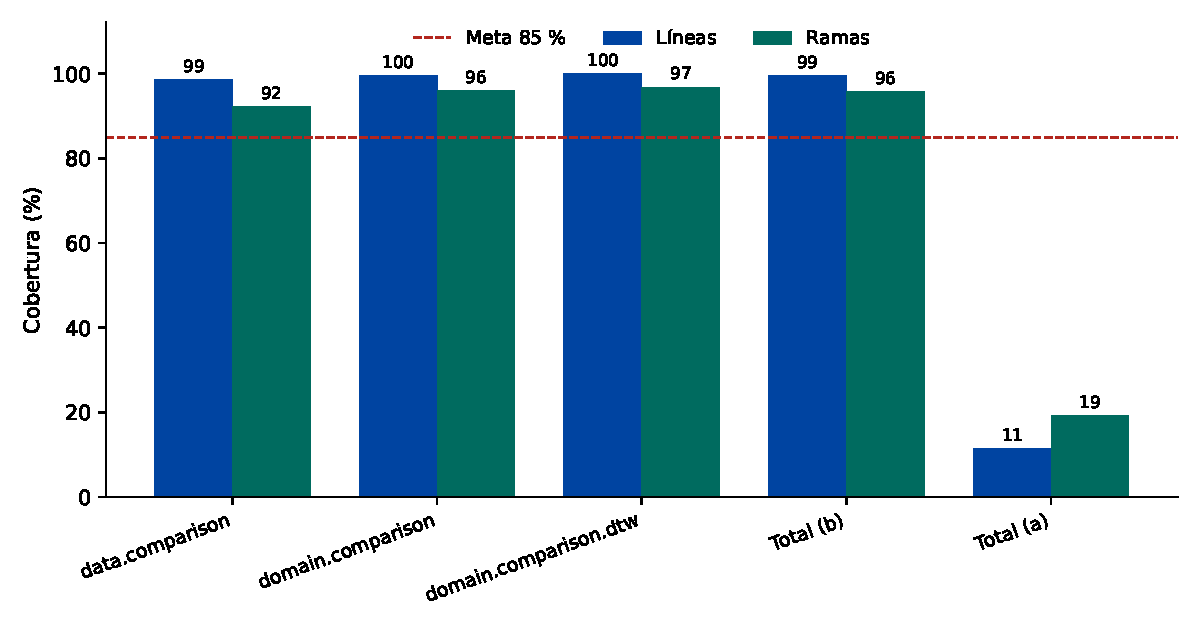
\includegraphics[width=\linewidth]{docs/cobertura/resumen_cobertura.pdf} % TODO: ruta
  \caption{Cobertura de líneas y ramas del alcance declarado (b), por paquete, frente a la
    meta del 85\,\%. Las dos barras finales muestran los totales de (b) y de (a).}
  \label{fig:cobertura}
\end{figure}

Sobre el alcance declarado (b) la cobertura es de \textbf{99,5\,\% de líneas (1127/1133)} y
\textbf{95,8\,\% de ramas (683/713)}, por encima de la meta del 85\,\% en ambas métricas.
% Medición del 2026-11-14 (docs/informe-cobertura/evidencia/medicion_2026-11-14.md).
El módulo completo (a) queda en 11,4\,\% de líneas y 19,2\,\% de ramas, valor que, como se
explicó, refleja la proporción de código de interfaz y de integración con la plataforma y
no es comparable con (b).

La tabla~\ref{tab:cobertura-clases} desglosa (b) por archivo fuente. Las ramas que
quedan sin cubrir se revisaron una por una en el reporte HTML y corresponden a tres
categorías: (i)~desempates internos de la recurrencia DTW que, con la distancia angular
real, no pueden alcanzarse sin construir una métrica artificial (\texttt{Dtw}, 4~ramas);
(ii)~operandos de condiciones booleanas compuestas cuyo cortocircuito ya fue ejercitado
por otro operando equivalente (\texttt{DefaultAngleExtractor}, \texttt{ErrorAttributor},
\texttt{ShapeSimilarity}, \texttt{DtwMovementComparator}); y (iii)~ramas defensivas que
protegen invariantes ya garantizadas por el llamador o por una validación previa
(\texttt{PeakValleyRepetitionSegmenter}, \texttt{ReferenceAlignment},
\texttt{ReferenceRepSelector}, la segunda comprobación de valores no finitos en
\texttt{ReferenceJsonParser}, que kotlinx.serialization rechaza antes, las tres de
\texttt{AdaptiveRestRepetitionSegmenter} que suponen un cuadro de cierre sin conductor
válido, y el caso de colección vacía del \texttt{maxOf} sobre las plantillas constantes de
\texttt{RepShapeGate}). Ninguna corresponde a comportamiento observable no probado.
% Clasificación revisada contra el XML en la re-medición del 2026-11-14 (30 ramas).

Respecto de los artefactos del compilador de Kotlin: JaCoCo~0.8.15 filtra las ramas que el
compilador agrega para \texttt{when} exhaustivos, argumentos por defecto, corrutinas,
funciones \texttt{inline} y los métodos sintetizados de las \texttt{data class}
(\texttt{equals}, \texttt{hashCode}, \texttt{toString}, \texttt{copy},
\texttt{componentN}); se verificó en el XML que estos últimos no aparecen en ninguna de las
13~\texttt{data class} del alcance, por lo que el conteo de ramas de (b) corresponde a
ramas escritas en el código fuente.

\begin{table}[htbp]
  \centering
  \caption{Cobertura del alcance declarado (b) por archivo fuente. ``Ramas sint.'' cuenta
    ramas no cubiertas en métodos sintetizados por el compilador de Kotlin (0 en todos los
    casos: JaCoCo las filtra).}
  \label{tab:cobertura-clases}
  \scriptsize
  % Generado por docs/cobertura/gen_cobertura.py — no editar a mano.
% Requiere \usepackage{booktabs}. Última columna: ramas no cubiertas que pertenecen
% a métodos sintetizados por el compilador de Kotlin (equals/hashCode/toString/copy/componentN).
\begin{tabular}{@{}llrrrrr@{}}
\toprule
\textbf{Paquete} & \textbf{Archivo} & \textbf{Líneas} & \textbf{\%} & \textbf{Ramas} & \textbf{\%} & \textbf{Ramas sint.} \\
\midrule
data.comparison & DtwMovementComparator.kt & 112/113 & 99,1\,\% & 44/48 & 91,7\,\% & 0 \\
data.comparison & ReferenceJson.kt & 96/98 & 98,0\,\% & 28/30 & 93,3\,\% & 0 \\
domain.comparison & AdaptiveRestRepetitionSegmenter.kt & 207/207 & 100,0\,\% & 130/133 & 97,7\,\% & 0 \\
domain.comparison & AngleDefinition.kt & 24/24 & 100,0\,\% & 20/20 & 100,0\,\% & 0 \\
domain.comparison & AngleExtractor.kt & 29/29 & 100,0\,\% & 26/30 & 86,7\,\% & 0 \\
domain.comparison & AngleFrame.kt & 9/9 & 100,0\,\% & 4/4 & 100,0\,\% & 0 \\
domain.comparison & Comparisons.kt & 0/0 & — & 0/0 & — & 0 \\
domain.comparison & CorrectionHint.kt & 12/13 & 92,3\,\% & 0/0 & — & 0 \\
domain.comparison & ErrorAttributor.kt & 80/80 & 100,0\,\% & 54/58 & 93,1\,\% & 0 \\
domain.comparison & ExerciseReference.kt & 15/15 & 100,0\,\% & 4/4 & 100,0\,\% & 0 \\
domain.comparison & MovementComparator.kt & 13/13 & 100,0\,\% & 0/0 & — & 0 \\
domain.comparison & MovementPatternCatalog.kt & 90/91 & 98,9\,\% & 22/22 & 100,0\,\% & 0 \\
domain.comparison & PeakValleyRepetitionSegmenter.kt & 109/109 & 100,0\,\% & 63/66 & 95,5\,\% & 0 \\
domain.comparison & ReferenceAlignment.kt & 57/57 & 100,0\,\% & 42/44 & 95,5\,\% & 0 \\
domain.comparison & ReferenceProvenance.kt & 4/4 & 100,0\,\% & 2/2 & 100,0\,\% & 0 \\
domain.comparison & ReferenceRepSelector.kt & 49/50 & 98,0\,\% & 62/64 & 96,9\,\% & 0 \\
domain.comparison & RepMetricsSink.kt & 1/1 & 100,0\,\% & 0/0 & — & 0 \\
domain.comparison & RepShapeGate.kt & 39/39 & 100,0\,\% & 29/30 & 96,7\,\% & 0 \\
domain.comparison & RepetitionSegmenter.kt & 4/4 & 100,0\,\% & 0/0 & — & 0 \\
domain.comparison.dtw & Dtw.kt & 104/104 & 100,0\,\% & 94/98 & 95,9\,\% & 0 \\
domain.comparison.dtw & LocalDistance.kt & 19/19 & 100,0\,\% & 26/26 & 100,0\,\% & 0 \\
domain.comparison.dtw & ShapeSimilarity.kt & 54/54 & 100,0\,\% & 33/34 & 97,1\,\% & 0 \\
\bottomrule
\end{tabular}
 % TODO: ruta
\end{table}

\subsubsection{Cumplimiento del umbral}

La meta no es solo un número reportado: la tarea \texttt{jacocoComparisonVerification}
declara una regla de JaCoCo sobre el alcance (b) con mínimo 0,85 para los contadores de
líneas y de ramas, y hace fallar el build si cualquiera de los dos baja. Se comprobó el
mecanismo elevando temporalmente el mínimo de ramas a 0,99: la tarea falló con el mensaje
\emph{``branches covered ratio is 0.95, but expected minimum is 0.99''}. La verificación se
ejecuta con:

\begin{verbatim}
.\gradlew :app:jacocoComparisonVerification
\end{verbatim}

% TODO: decidir si se menciona la integración continua. Hoy el repositorio móvil no tiene
% workflow; el equivalente sería un job de GitHub Actions que ejecute
% `gradlew testAwsDebugUnitTest jacocoComparisonVerification jacocoAwsDebugUnitTestReport`
% y publique app/build/reports/jacoco/** como artefacto (no requiere el modelo .tflite ni
% local.properties, porque las pruebas son JVM puras).
